\cleardoublepage

\chapter{Introducción}
\label{makereference}

Este proyecto tiene como objetivo predecir, a través de herramientas informáticas, la radiación solar en un punto teniendo en cuenta factores geográficos y meteorológicos.

% Mirar descripción inicial TFG y Drive

\begin{figure}[htb]%t=top, b=bottom, h=here
	
	\begin{center}
		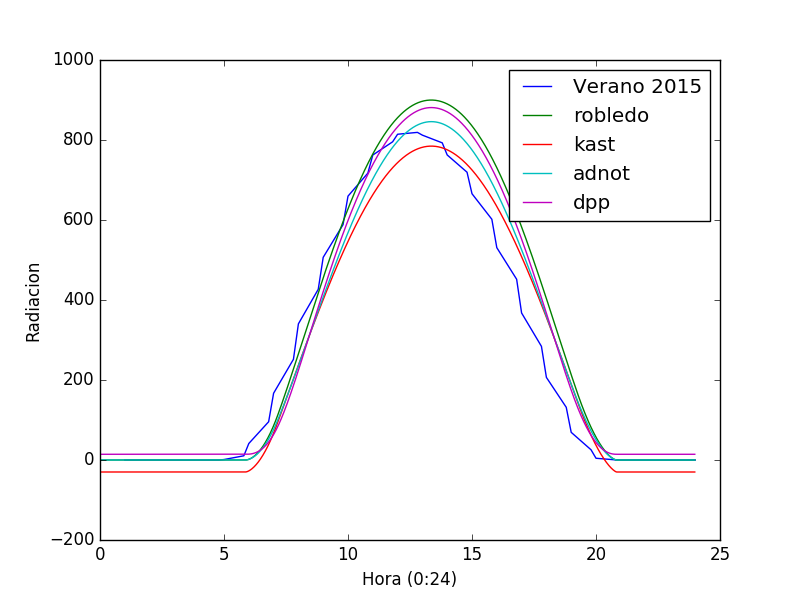
\includegraphics[height=2.5in]{figures/verano2015.png}
		\caption{Modelo verano 2015}
	\end{center}
    
    \label{figure1}
\end{figure}

% +--------------------------------------------------------------------+
% |To create cross-references to figures, tables and segments
% |of text, LaTeX provides the following commands:
% |   \label{marker}
% |   \ref{marker}
% |   \pageref{marker}
% | where {marker} is a unique identifier.
% |
% | In the line above, we use \label{figure1} to mark a location
% | we wish to refer to later.  LATEX replaces \ref by the number of
% | the chapter, section, subsection, figure, or table after which the
% | corresponding \label command was issued. \pageref prints the page
% | number of the page where the \label command occurred.
% |
% +--------------------------------------------------------------------+

\section{Motivación}
\label{makereference1.1}

Hoy en día es cada vez más importante el uso de \textbf{las energías renovables} y así utilizar cada vez menos los combustibles fósiles. Además de la abundancia de estas energías y su gran aprovechamiento, la causa principal es que estas no producen gases de efecto invernadero que son los causantes del \textbf{cambio climático}, ni tampoco producen emisiones contaminantes. Además de la ventaja más importante actualmente, que es su ayuda en contra del cambio climático, son inagotables o no generan residuos difíciles de trata. Aunque también tiene algunos inconvenientes como por ejemplo, el gran impacto visual que tienen y las grandes cantidades de terreno que se necesitan para poder conseguir una cantidad significante de energía, además de que no siempre se obtiene la misma cantidad de energía, depende por ejemplo de la cantidad de sol.

Este último inconveniente es el que hace que las compañías productoras y distribuidoras son reacias al no saber la capacidad de producción de antemano.




\section{Breve descripción del sistema}
\label{makereference1.2}

Este sistema cuenta con cuatro grandes módulos de trabajo para llevar a cabo su función: nodo, servidor de datos, servidor de resultados y visualizador de datos.

\subsection{Nodo}
\label{makereference1.2.1}
Encargado de recoger los datos necesarios, está formado por distintos sensores que recogen la información meteorológica necesaria y una pequeña placa programable encargada de enviar esta información al \textbf{servidor de datos}.

\subsection{Servidor de datos}
\label{makereference1.2.2}
El \textbf{servidor de datos}, es el encargado de recibir, almacenar y distribuir la información obtenida por el \textbf{nodo}.

\subsection{Servidor de cálculo}
\label{makereference1.2.3}
Tiene como función recoger la información almacenada del servidor de datos, procesarla para obtener la predicción y enviarla al \textbf{visualizador de datos}. Puede estar, o no, en la misma máquina que el servidor de datos.

\subsection{Sistema de visualización}
\label{makereference1.2.4}
El sistema de visualización de datos elegido es ThingSpeak, una aplicación de código abierto que permite llevar un registro de los datos que se desean. Permite representarlos y estudiarlos.

\begin{figure}[htb]
    \begin{center}
        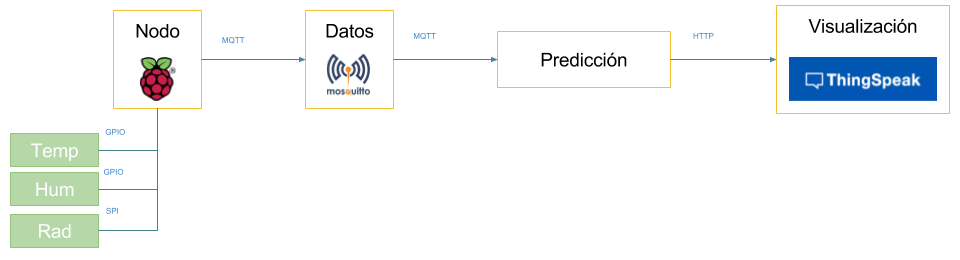
\includegraphics[height=2in]{figures/diagrama-sistema.png}
        \caption{Diagrama de los componentes del sistema con sus protocolos de comunicación.}
    \end{center}
    \label{diagrama-sistema}
\end{figure}
